\documentclass{article}

\usepackage{microtype}
\usepackage{graphicx}
\usepackage{booktabs}
\usepackage{multirow}
\usepackage{amsmath}
\usepackage{amssymb}
\usepackage{xcolor}
\usepackage{hyperref}
\usepackage[preprint]{icml2026}
\usepackage[capitalize,noabbrev]{cleveref}

\makeatletter
\renewcommand{\ICML@preprint}{\textit{11-777 Midterm Project Report, Fall 2026.}}
\makeatother

\icmltitlerunning{Efficient Multimodal Reasoning: Midterm Report}

\begin{document}

\twocolumn[
  \icmltitle{\texorpdfstring{Efficient Multimodal Reasoning\\[0.25em]
  \large 11-777 Midterm Report, Team 7}
  {Efficient Multimodal Reasoning: 11-777 Midterm Report, Team 7}}

  \begin{icmlauthorlist}
    \icmlauthor{Nikkita Batra (nbatra)}{cmu}
    \icmlauthor{Arjun Shah (aashah2)}{cmu}
    \icmlauthor{Alvin Wang (alvinw2)}{cmu}
    \icmlauthor{Lindy Zhang (lindyz)}{cmu}
  \end{icmlauthorlist}

  \icmlaffiliation{cmu}{Carnegie Mellon University, Pittsburgh, Pennsylvania, USA}
  \icmlcorrespondingauthor{Nikkita Batra}{nbatra@andrew.cmu.edu}
  \icmlkeywords{multimodal machine learning, efficient inference, routing, token budgets}
  \vskip 0.3in
]

\printAffiliationsAndNotice{}

\begin{abstract}
Omni-modal models answer questions about images, audio, and text, but raw images
and audio dominate their inference cost. We study how such a model should
allocate computation across modalities without losing accuracy, using
Qwen2.5-Omni-3B on OmniBench. The technical challenge is that the value of each
modality changes from item to item and is entangled with how the other modalities
are represented, and that cheap substitutes (captions, transcripts, compressed
inputs) may silently drop the information a question needs. We implement one
baseline per research idea and evaluate each on held-out items with accuracy
averaged over option permutations, which removes a strong answer-position bias.
(1) A learned representation router has large headroom (a per-item oracle reaches
69\% accuracy at a third of the full-input cost, versus 45\% for the full input),
but a logistic-regression router does not beat mixing fixed configurations,
because its features predict item difficulty rather than which modality helps.
(2) Visual tokens saturate after about 64 per image while audio tokens carry most
of the remaining utility; image and audio interact strongly, and per-audio-type
budget tables overfit. (3) Text surrogates match the raw input only when they are
the benchmark's reference surrogates (a large-VLM caption and human-written audio
transcripts): surrogates generated at test time captions and audio descriptions lose 7.5 points,
mostly on music, and generating them costs about 25$\times$ more than answering from
the raw inputs. Together, these results motivate item-level allocation that accounts for cross-modal interactions, along with more appropriate audio surrogates.
\end{abstract}

\noindent\textbf{Code:} \href{https://github.com/alvinwang1/multimodal-reasoning-project/}{github.com/alvinwang1/multimodal-reasoning-project}.

% ===========================================================================
\section{Introduction}
\label{sec:intro}

Multimodal models increasingly reason jointly over vision, audio, and language
within one network~\citep{lu2024unifiedio2,zhan2024anygpt,sun2024videosalmonn,xu2025qwen25omni}.
Their cost is dominated by the non-text modalities: in our setting an image becomes
about 700 tokens and a 10-second clip about 250, while the question and options
take roughly 130. Whether such systems run on phones, wearables, and assistive
devices, or only in data centers, depends on how much of this computation is
actually needed. Latency also matters in interactive settings, where a late answer
has little value.

Reducing this cost is hard for three reasons that prior work leaves open. First,
the useful modality changes per item: some questions are answered by the audio,
some by the image, and some by neither. Second, modalities interact, so the value
of a visual token depends on whether and how the audio is represented. Third,
cheaper representations (fewer tokens, or text in place of raw signals) can
silently drop exactly the evidence a question needs, and their own production may
cost more than it saves. Existing token-compression work mostly targets a single
modality or a fixed compression strategy, and it rarely asks when a different representation type, such as a caption or transcript, is the cheaper
sufficient input.

In this paper we build and analyze baselines for three research ideas from our
proposal, all on Qwen2.5-Omni-3B and OmniBench~\citep{li2025omnibench}:
\textbf{Idea~1}, a learned router that chooses, per item, among raw, surrogate, and
mixed input representations; \textbf{Idea~3}, a controlled study of the marginal
utility of image and audio tokens under budgets; and \textbf{Idea~4}, replacing raw
modalities with model-generated text surrogates and counting their
generation cost. We keep the numbering of our proposal. Because our Assignment~2 analysis found that
OmniBench's answers sit at position ``D'' for 49\% of items while the model prefers
``B'', every accuracy in this report is averaged over three option orders.

Our contributions are diagnostic: (1) we show that per-item routing has 15 points of
accuracy headroom at a third of the cost, and that a standard learned router fails
to capture it because its features measure item difficulty rather than modality
benefit; (2) we measure the marginal utility of visual and audio tokens and a large
positive image--audio interaction, and show that coarse per-audio-type budgets
overfit; (3) we show that text surrogates beat raw inputs only when they are the
benchmark's reference surrogates, partly because its human-written audio descriptions
name the answer, and that
generating them costs far more than it saves. Each failure motivates a concrete
method for the final report.


% ===========================================================================
\section{Related Work}
\label{sec:related}

\paragraph{Omni-modal models.} Unified-IO~2~\citep{lu2024unifiedio2} and
AnyGPT~\citep{zhan2024anygpt} map heterogeneous inputs into one token stream;
video-SALMONN~\citep{sun2024videosalmonn} and Qwen2.5-Omni~\citep{xu2025qwen25omni}
connect pretrained vision and audio encoders to a language model.
OmniBench~\citep{li2025omnibench} evaluates joint image--audio--text reasoning and
supplies the reference surrogates we use: image captions generated by
InternVL-2-76B and human-annotated audio transcripts (descriptions for non-speech
audio). It also reports a textual-approximation setting in which these surrogates
replace the raw inputs.

\paragraph{Token efficiency.} Vision-language
compression prunes or merges visual tokens using cross-modal alignment
(MADTP;~\citealp{cao2024madtp}), attention statistics
(FastV;~\citealp{chen2024fastv}; FitPrune;~\citealp{ye2025fitprune}), merging
(LLaVA-PruMerge;~\citealp{shang2025llavaprumerge}), coarse-to-fine projection
(TokenPacker;~\citealp{li2025tokenpacker}), nested token sets
(Matryoshka;~\citealp{cai2024matryoshka}), or faster encoders
(FastVLM;~\citealp{vasu2025fastvlm}). For audio--visual inputs,
OmniSIFT~\citep{ding2026omnisift} compresses the two modalities asymmetrically,
OmniSelect~\citep{yang2026omniselect} picks a modality-specific pruning strategy per
input, OmniPack~\citep{su2026omnipack} combines structural and query-guided
compression, and HeadRouter~\citep{he2026headrouter} shows that audio token
importance depends on the task. Unlike these methods, which choose \emph{how much}
of each modality to keep, Idea~1 chooses among representation \emph{types}, and
Idea~3 measures the marginal utility and interaction of each modality's tokens
directly rather than proposing another pruning rule.

\paragraph{Routing and cascades (Idea 1).} FrugalGPT~\citep{chen2023frugalgpt}
cascades language models by confidence, and RouteLLM~\citep{ong2024routellm} learns
to route queries between a strong and a weak model from preference data. We route
among input representations of one frozen model instead of among models; our
failure analysis connects to known miscalibration of neural
confidence~\citep{guo2017calibration}.

\paragraph{Text surrogates (Idea 4).} Describe-then-answer pipelines such as
PICa~\citep{yang2022pica} and Socratic Models~\citep{zeng2023socratic} convert
perception into text and let a language model reason over it. We use
Whisper~\citep{radford2023whisper} for speech and the backbone itself for captions
and audio descriptions. Whisper is known to hallucinate text, particularly during
non-vocal segments~\citep{koenecke2024careless}; we quantify this failure on
non-speech audio. OmniBench evaluates its offline reference surrogates as textual
approximations; to our knowledge, we are the first to replace them with surrogates
generated at test time by the answering model and an ASR system, and to count their
generation cost.

\paragraph{Evaluation robustness.} Multiple-choice evaluation of language models
is sensitive to option order and letter
priors~\citep{zheng2024mcq,pezeshkpour2024order}; we average over permutations for
this reason. Modality imbalance and greedy reliance on one
modality~\citep{wu2022greedy,peng2022ogm}, and interaction
measures~\citep{hessel2020emap,liang2023pid}, inform our Idea~3 analysis.

% ===========================================================================
\section{Problem Statement}
\label{sec:problem}

An item is $x=(q,O,v,a)$ with question $q$, options $O=(o_1,\dots,o_4)$, image $v$,
and audio $a$; the label $y\in\{1,\dots,4\}$ is the correct option. A
\emph{representation} $r=(r_v,r_a)\in\mathcal{R}$ specifies how each modality is
presented: raw, compressed to a token budget, replaced by a text surrogate (the
dataset's reference caption $c_v$ or transcript $t_a$, or a caption $\hat c_v$ or
transcript $\hat t_a$ that we generate), or omitted. A frozen model $f_\theta$ (Qwen2.5-Omni-3B) answers with
the option letter it gives the highest probability. Because its answer can depend on
where the correct option is placed, we ask every question under three option orders
$\pi$ (the original order and two seeded shuffles) and map each answer back to the
original options. Accuracy is the fraction of orders answered correctly,
\begin{equation}
\mathrm{acc}(x,r)=\frac{1}{3}\sum_{\pi=1}^{3}\mathbf{1}\big[\hat y_\pi(x,r)=y\big],
\end{equation}
where $\hat y_\pi(x,r)$ is the model's answer when item $x$ is shown with
representation $r$ in order $\pi$, and $\mathbf{1}[\cdot]$ is 1 for a correct answer
and 0 otherwise, so $\mathrm{acc}(x,r)\in\{0,\tfrac13,\tfrac23,1\}$. The cost
$C(x,r)$ is the number of input tokens divided by the tokens of the full raw input (so
the full input costs 1), plus the cost of producing the representation when it must
be generated, such as writing a caption. A policy $\rho$ picks a representation for
each item, and we want policies that are accurate and cheap on average:
\begin{equation}
\max_{\rho}\ \ \overline{\mathrm{acc}}(\rho)\;-\;\lambda\,\overline{C}(\rho),
\end{equation}
where the bars denote averages over items. The weight $\lambda\ge0$ sets how much
accuracy we are willing to give up per unit of cost: $\lambda=0$ ignores cost, larger
$\lambda$ favors cheaper representations, and sweeping $\lambda$ traces an
accuracy--cost curve.
Idea~1 learns $\rho$ over a fixed set of representation types; Idea~3 studies
$\mathcal{R}$ as a grid of token budgets $(b_v,b_a)$; Idea~4 adds generated
surrogates to $\mathcal{R}$ and includes their generation cost in $C$.

% ===========================================================================
\section{Experimental Methodology}
\label{sec:method}

\paragraph{Data.} OmniBench has 1,142 four-option questions, each with an image, an
audio clip (speech, sound event, or music), an image caption generated by
InternVL-2-76B, and a human-annotated audio transcript; for sound events and music,
the ``transcript'' is a human-written description of the audio. One item with duplicate options is excluded. For Ideas~1 and~4 we use
300 items balanced by audio type: \textbf{180 train} (the 90-item Assignment~2
subset plus 90 new items) and \textbf{120 test} items not seen before. Idea~3 uses
the Assignment~2 subset as its development set and a disjoint, seeded 90-item test
set with the same balance.

\paragraph{Model and scoring.} Qwen2.5-Omni-3B (thinker only, text output) scores
each item with one forward pass by a softmax over the logits of the letters A--D.
Images are resized to at most 768 visual tokens (mean 700); audio costs 25 tokens
per second. We log input tokens by modality and forward latency. Runs used an Apple
M2 Max (bf16), a V100 (fp32), and an L4 (bf16). Predictions agree on 97.5\% of
1,890 shared passes between the M2 Max and the V100, and on 81\% of the 1,800
Idea~4 passes between the M2 Max and the L4; the lower agreement there comes from
slightly different generated text.

\paragraph{Evaluation.} We report test accuracy averaged over three option orders,
cost as input tokens relative to the full raw input, and latency. Differences are
tested with paired bootstrap confidence intervals over items and sign-flip or
Wilcoxon tests. With 40 test items per audio type, per-type differences below about
8 points are within noise. As upper and lower references we use a per-item
\emph{oracle} (the cheapest representation that is best on that item) and an
always-``D'' baseline (43\% on the Assignment~2 subset).

% ===========================================================================
\section{Idea 1: Adaptive Representation Routing}
\label{sec:idea1}

\subsection{Initial Implementation}

\paragraph{Idea.} In Assignment~2, the cheapest representation that still answered
an item correctly varied a lot from item to item. Idea~1 trains a router that picks
one of seven representations for each item: image+audio (full), image+transcript,
caption+audio, caption+transcript, image only, audio only, or question only.
Methods such as OmniSelect~\citep{yang2026omniselect} decide how much of each
modality to prune; our router instead decides which type of input to use.

\paragraph{Labels.} For training item $i$ and representation $r$, the label is
$y_{i,r}=\mathrm{acc}(x_i,r)$, the fraction of the three option orders answered
correctly. Computing all labels took 6,300 forward passes (300 items, 7
representations, 3 orders).

\paragraph{Features.} The router sees only cheap signals: a \emph{probe} pass with
caption+transcript (its sorted option probabilities, the gap between the top two,
and the entropy); the question's Sentence-BERT embedding~\citep{reimers2019sentencebert},
reduced to 16 dimensions with PCA fitted on train; the caption and transcript
lengths; and the audio type.

\paragraph{Model.} One logistic regression per representation predicts $\hat p_r(x)$,
the probability that $r$ answers item $x$ correctly. Because the labels are
fractions, we train with cross-entropy on soft labels plus an L2 penalty:
\begin{equation}
\mathcal{L}_r=-\sum_i\Big[y_{i,r}\log\hat p_r(x_i)+(1-y_{i,r})\log\big(1-\hat p_r(x_i)\big)\Big]+\alpha\|w_r\|^2 .
\end{equation}
The first term pulls $\hat p_r$ toward the label. The second keeps the weights small,
which matters with only 180 training items. The router then picks the
representation with the best predicted accuracy minus a cost penalty:
\begin{equation}
\rho_\lambda(x)=\arg\max_{r}\ \big[\hat p_r(x)-\lambda\,C_r(x)\big].
\end{equation}
When the probe is used, its cost is added to every choice except
caption+transcript, whose answer the probe already provides. We train four
variants: with or without the probe, and with or without the audio type, which a
real system would have to infer. $\lambda$ is tuned on train.

\paragraph{Baselines.} We compare against each fixed representation; the convex hull
of the fixed representations, which is what randomly mixing them achieves at any
cost; a confidence cascade~\citep{chen2023frugalgpt} that answers from
caption+transcript and switches to image+transcript or the full input when the top
probability is below $\tau$ (tuned on train); and the oracle.

\subsection{Results and Discussion}

\begin{table}[t]
\caption{Idea~1 on the 120 test items: accuracy (mean over 3 option orders) and cost
(input tokens relative to the full input). Router and cascade operating points are
tuned on train.}
\label{tab:idea1}
\centering\small
\setlength{\tabcolsep}{4pt}
\begin{tabular}{lcc}
\toprule
Method & Acc.\ (\%) & Cost \\
\midrule
Image+Audio (full)                  & 45.3 & 1.00 \\
Image+Transcript                    & \textbf{54.2} & 0.78 \\
Caption+Audio                       & 41.1 & 0.58 \\
Caption+Transcript                  & 45.0 & 0.36 \\
Audio only / Image only             & 38.9 / 35.0 & 0.36 / 0.75 \\
Question only                       & 30.3 & 0.12 \\
\midrule
Cascade $\to$ Image+Transcript ($\tau{=}.65$) & 49.7 & 0.57 \\
Router, probe                       & 44.2 & 0.65 \\
Router, probe-free                  & 44.4 & 0.57 \\
Router, probe-free, no audio type   & 45.0 & 0.53 \\
\midrule
Oracle (per item)                   & 69.2 & 0.33 \\
\bottomrule
\end{tabular}
\end{table}

\begin{figure}[t]
\centering
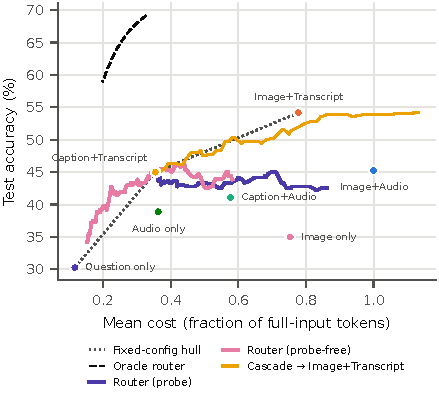
\includegraphics[width=\columnwidth]{figures/router_curve.pdf}
\caption{Idea~1 test accuracy vs.\ cost. Routers and the cascade trace curves as
$\lambda$ or $\tau$ varies; dots are fixed representations; the dotted line is their
convex hull (random mixing at matched cost); the dashed line is the oracle.}
\label{fig:idea1-curve}
\end{figure}

\paragraph{Large headroom, no gain yet.} The oracle reaches 69.2\% at a third of
the full-input cost, 15 points above the best fixed choice, image+transcript
(54.2\%; \cref{tab:idea1}). None of the learned routers comes close. At their
train-tuned settings they score 44--46\%, below the hull at the same cost
(\cref{fig:idea1-curve}); the probe-free router, for example, is 5.2 points below it
at cost 0.57. The cascade lands on the hull but not above it. Routing helps only at
very low budgets, where the probe-free router beats the hull by up to 5.9 points
around cost 0.2 by sending easy-looking items to question only or audio only. The
probe router cannot reach this region because the probe alone costs 0.36, and it
rarely escalates: 59 of 120 items stay on caption+transcript.

\begin{table}[t]
\caption{Idea~1 feature ablation (test). Each row trains the same per-representation
routers on a different feature set; $\lambda$ is tuned on train. ``Max gain'' is the
best improvement over the fixed-representation hull across all $\lambda$; ``rank''
is the mean per-item Spearman correlation between predicted and true accuracy across
the seven representations.}
\label{tab:idea1-ablation}
\centering\small
\setlength{\tabcolsep}{3pt}
\begin{tabular}{lcccc}
\toprule
Features & Acc. & Cost & Max gain & Rank \\
\midrule
Probe only (5)                    & 48.9 & 0.82 & $+0.7$ & .24 \\
Probe + audio type (8)            & \textbf{50.3} & 0.83 & $+0.6$ & .16 \\
Question embedding only (16)      & 45.0 & 0.46 & $+5.3$ & .16 \\
Lengths + audio type (5)          & 48.3 & 0.58 & $+5.8$ & .10 \\
All but probe (21)                & 44.4 & 0.57 & $+5.9$ & .13 \\
All features (26)                 & 44.2 & 0.65 & $-0.4$ & .10 \\
\bottomrule
\end{tabular}
\end{table}

\paragraph{More features hurt.} The full router overfits (\cref{tab:idea1-ablation}):
with all 26 features it scores 44.2\%, compared with 50.3\% using only the probe and
the audio type. No feature set ranks the seven representations well within an item
(mean rank correlation 0.10--0.24). The largest low-budget gain comes from the
lengths and audio type, which suggests the router mostly learns whether an item is
easy enough to answer from the question alone, not which modality it needs. By
audio type, the probe-free router does reasonably on music (59.2\% vs.\ 66.7\% for
always using image+transcript) but poorly on sound events (37.5\% vs.\ 55.0\%), where
the answer depends on the raw audio or image.

\paragraph{Why the router fails.} We see three causes. (i) \emph{It learns difficulty,
not modality.} The strongest feature is the probe's entropy, and its weight is
negative for every representation ($-0.21$ to $-0.57$). The router therefore learns
which items are hard for every input, not which input would fix a given item. On
solvable test items it picks a best representation only 48\% of the time. (ii)
\emph{It is overconfident.} When it predicts 0.67 for its choice, that choice is right
only 43\% of the time~\citep{guo2017calibration}. The probe is often confidently
wrong (mean top probability 0.71 on high-regret items), so escalation rarely
triggers. As a result, the router mostly picks caption+transcript or
image+transcript, while the oracle's choices are spread over all seven
(\cref{fig:idea1-confusion}). (iii) \emph{The labels are noisy.} 13\% of test items
are never answered correctly, and on many others several representations tie at
chance level. The oracle's cheapest-best choice is question only on 45 items, mostly
by luck.

Two examples show the pattern. For item 1020 (\emph{``Why did the woman laugh?''}),
the router picks audio only and is wrong in all three orders, while every
representation that includes the image is right in all three. For item 1047
(\emph{``Which type of instrument can you tell from both the image and audio?''}),
it picks image only and fails; only representations with the human audio
description succeed, and even the full raw input fails. Removing the audio type does
not hurt (45.0\% vs.\ 44.4\%), which matches Idea~3's finding that audio type is too
coarse a signal.

\begin{figure}[t]
\centering
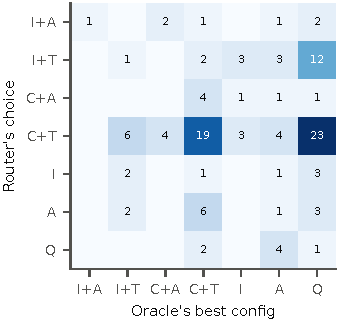
\includegraphics[width=\columnwidth]{figures/router_confusion.pdf}
\caption{Idea~1: router choice (probe variant, train-tuned $\lambda$) vs.\ the
oracle's best representation on the 120 test items. The router concentrates on two
text-heavy representations; many of the oracle's ``question only'' choices are
chance-level ties.}
\label{fig:idea1-confusion}
\end{figure}

\subsection{Updated Research Idea}

The router should predict which representation is \emph{better}, not whether each
one is correct on its own. We plan four changes. (a) \emph{Pairwise training.} We
will learn a score $s(x,r)$ with a pairwise loss:
\begin{equation}
\begin{aligned}
\mathcal{L}_{\text{pair}}
&= \sum_i
\sum_{\substack{r,r':\\ y_{i,r}>y_{i,r'}}}
(y_{i,r}-y_{i,r'}) \\
&\quad \cdot
\log\left(
1+\exp\left[
s(x_i,r')-s(x_i,r)
\right]
\right).
\end{aligned}
\end{equation}
For each pair where $r$ did better than $r'$ on item $i$, the loss is small only if
$s$ ranks $r$ above $r'$. Each pair is weighted by how much better $r$ was, so ties
and unsolvable items add nothing, and a shared ``this item is hard'' signal cancels
out. (b) \emph{Cleaner labels.} We will use correctness under all three orders and
$\log p(\text{gold})$ instead of chance-level wins. (c) \emph{Disagreement
features.} We will add features from cheap image-only and audio-only passes, since
the failures above are items where the two modalities point to different answers.
(d) \emph{Calibration.} We will temperature-scale the probe before using its
confidence. We will also add Idea~3's budget cells to the menu, so the router can
choose a 64-token image instead of none or 700.

In course terms, the router decides how to fuse the modalities: all raw signals
together, a raw signal plus a translated one, or translations only. We will also
test it as a contextual bandit, where only the outcome of the chosen representation
is observed. The updated router must beat the fixed-representation hull at matched
cost, which no midterm variant does except at very low budgets.

% ===========================================================================
\section{Idea 3: Marginal Utility of Modality Budgets}
\label{sec:idea3}

\subsection{Motivation and Initial Implementation}

Assignment~2 suggested that image and audio matter by different amounts, and that
this flips with audio type: the image helped on speech, while audio mattered more on
sound events. If so, a single fixed input recipe wastes computation, and tokens
should be allocated per audio type. Idea~3 tests this by measuring how much accuracy
each extra image or audio token buys, and whether these numbers are stable enough to
set a budget policy.

\paragraph{Budget cells.} A cell $b=(b_v,b_a)$ limits the image to $b_v\in\{0,64,256,768\}$
visual tokens by resizing ($\text{max\_pixels}=28^2 b_v$) and keeps the first
fraction $b_a\in\{0,\tfrac14,\tfrac12,1\}$ of the audio (at least 1\,s; 25 tokens per
second). Three more cells replace the image and/or audio with the caption or
transcript. Each cell is scored by
\begin{equation}
s(x;b)=\frac{1}{3}\sum_{\pi=1}^{3}\log p_\theta\big(y\mid x\text{ at budget }b,\ \text{order }\pi\big),
\end{equation}
the log-probability of the correct answer, averaged over the three orders. It is 0
when the model is certain and correct, and it drops as probability moves away from
the right answer. Because it changes smoothly, it shows small differences that 0/1
accuracy on 90 items would miss; we report accuracy as well. The cost $c(x;b)$ is
the number of input tokens.

\paragraph{Modality attribution.} Let $s_{va}$, $s_v$, $s_a$, and $s_{\varnothing}$
be the scores with both modalities, image only, audio only, and neither. The
per-item Shapley contributions~\citep{shapley1953value,lundberg2017shap} are
\begin{align}
\phi_v(x)
&=
\frac{1}{2}
\left[
(s_v-s_{\varnothing})
+
(s_{va}-s_a)
\right],\\
\phi_a(x)
&=
\frac{1}{2}
\left[
(s_a-s_{\varnothing})
+
(s_{va}-s_v)
\right],
\end{align}
and the interaction~\citep{hessel2020emap} is
\begin{equation}
I(x)=s_{va}-s_v-s_a+s_{\varnothing}.
\end{equation}
$\phi_v$ is the average gain from adding the image, with and without audio; $\phi_a$
is the same for audio. $I=0$ means the two contributions simply add up, $I>0$ means
the modalities help more together (synergy), and $I<0$ means they overlap or
interfere.

\paragraph{Marginal utility and policy.} The marginal utility of an image upgrade
(say from 64 to 256 tokens, with the audio fixed) is the score gain per extra token:
\begin{equation}
\mathrm{MU}_v=\frac{\overline{s}(\text{larger image})-\overline{s}(\text{smaller image})}{\overline{c}(\text{larger image})-\overline{c}(\text{smaller image})}.
\end{equation}
$\mathrm{MU}_a$ is defined the same way for audio. The baseline policy is a lookup
table: for each audio type $t$, it picks the cell with the best dev accuracy among
cells that cost at most a fraction $\beta$ of the full input,
\begin{equation}
\pi_\beta(t)=\arg\max_{b:\ \overline{c}_{\text{dev}}(b\mid t)\,\le\,\beta}\ \overline{\mathrm{acc}}_{\text{dev}}(b\mid t).
\end{equation}
For example, $\beta=0.4$ allows at most 40\% of the full input's tokens. We compare
it with a single global cell for all items, the full input, always answering ``D'',
and a per-item oracle that picks the cheapest cell correct in all three orders.

\paragraph{Setup.} We use the same model, prompt, and scoring as above. On each split
(90 dev, 90 test) we run the $4\times4$ grid and the three surrogate cells, 10,800
passes in total on a V100 (dev also has two centered-window audio cells). Because of
aspect-ratio rounding, the image budgets average 56, 240, and 694 tokens. As an
ablation, we also ran a \emph{time-stretching} grid on the 120-item test split of
Ideas~1 and~4: the image shrunk to $\{0,.1,.25,.5,1\}$ of its tokens and the audio
sped up, with pitch kept, to $\{0,.25,.5,1\}$ of its tokens (5,760 more passes).

\subsection{Results and Discussion}

\begin{table}[t]
\caption{Idea~3 test accuracy (\%, mean over 3 option orders; 30 items per audio
type) and mean input tokens for selected budget cells; dev accuracy (all types) in
the last column. $b_v$ = max image tokens, $b_a$ = audio fraction.}
\label{tab:idea3-grid}
\centering\small
\setlength{\tabcolsep}{3pt}
\begin{tabular}{lcccccc}
\toprule
Cell $(b_v,b_a)$ & Speech & Sound & Music & All & Tok. & Dev \\
\midrule
$(0,0)$ question only  & 21.1 & 24.4 & 41.1 & 28.9 &  127 & 31.1 \\
$(0,1)$ audio only     & 25.6 & 26.7 & 44.4 & 32.2 &  408 & 43.7 \\
$(768,0)$ image only   & 35.6 & 21.1 & 44.4 & 33.7 &  824 & 38.1 \\
$(64,1)$               & 46.7 & \textbf{45.6} & 48.9 & 47.0 &  466 & 44.4 \\
$(256,1)$              & 52.2 & 41.1 & 48.9 & 47.4 &  650 & 45.2 \\
$(768,1)$ full input   & \textbf{53.3} & 43.3 & 53.3 & 50.0 & 1104 & 45.2 \\
Caption+transcript     & 42.2 & 33.3 & 54.4 & 43.3 &  364 & 47.8 \\
Image+transcript       & \textbf{53.3} & 44.4 & \textbf{57.8} & \textbf{51.9} &  849 & \textbf{51.1} \\
\bottomrule
\end{tabular}
\end{table}

\begin{figure*}[t]
\centering
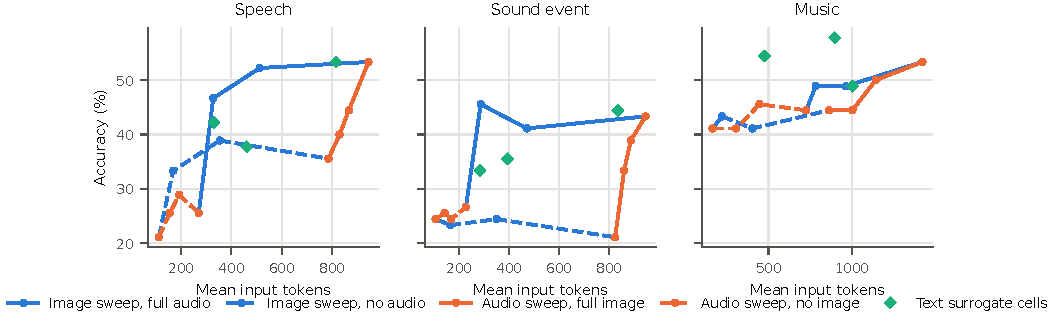
\includegraphics[width=\textwidth]{figures/idea3_marginal_curves_test.pdf}
\caption{Idea~3 test accuracy vs.\ mean input tokens along each budget sweep. Blue:
image budget $0\!\to\!64\!\to\!256\!\to\!768$ tokens with full (solid) or no (dashed)
audio; orange: audio fraction $0\!\to\!\tfrac14\!\to\!\tfrac12\!\to\!1$ with full
(solid) or no (dashed) image. Most of the image's value arrives in the first 64
tokens, and only when audio is present.}
\label{fig:idea3-curves}
\end{figure*}

\paragraph{Image tokens saturate early.} Most of the image's value comes from its
first 64 tokens (\cref{tab:idea3-grid,fig:idea3-curves}). With full audio, a
64-token image scores 47.0\% on test versus 50.0\% for the full image ($-3.0$, 95\%
CI $[-8.5,2.6]$) while using 42\% of the tokens; on dev the gap is only $-0.7$. Going
from no image to 64 tokens adds 14.8 points ($[7.0,23.0]$). The time-stretching grid
agrees: a 10\% image with full audio scores 45.6\%, the same as the full input
(45.3\%), with 37\% of the multimodal tokens. Favoring audio beats compressing both
modalities equally at every budget (45.6\% vs.\ 34.4\% at about 500 tokens).

\paragraph{Cut the audio, do not speed it up.} Keeping only the first half of the
clip works as well as the full clip (audio only: $-0.7$ points on dev, $+0.7$ on
test). Speeding the clip up to save the same tokens breaks speech: audio-only
accuracy on speech falls from 37.5\% to 21.7\% at 2$\times$ speed and to 12.5\% at
4$\times$, below chance. Music is unaffected (52.5--54.2\%). The audio encoder needs
speech at normal speed, so the way to save audio tokens is to choose which part to
keep (\cref{fig:idea3-stretch}). The same grid shows that on sound events, adding a
10\% image to the full audio raises accuracy from 26.7\% to 45.8\%, while on music
the image adds nothing.

\begin{figure}[t]
\centering
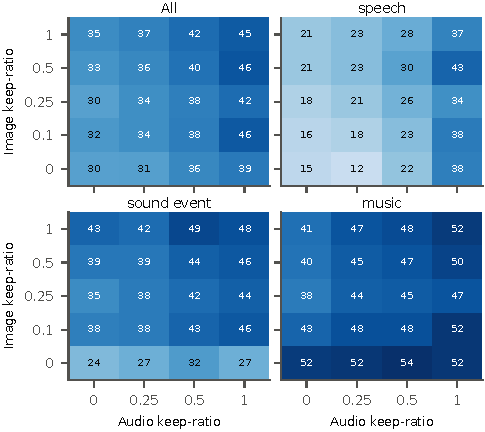
\includegraphics[width=\columnwidth]{figures/idea3_stretch_heatmaps.pdf}
\caption{Idea~3 time-stretching ablation on the 120-item test split of Ideas~1/4:
accuracy (\%) by image keep-ratio (rows) and audio keep-ratio (columns; audio sped
up to keep that share of its tokens). Speeding up speech destroys accuracy; a 10\%
image is enough on sound events.}
\label{fig:idea3-stretch}
\end{figure}

\begin{figure}[t]
\centering
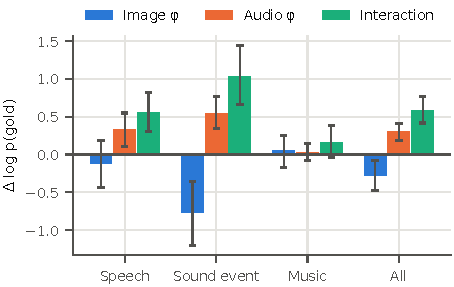
\includegraphics[width=\columnwidth]{figures/idea3_shapley.pdf}
\caption{Per-item Shapley values and interaction on $s=\log p(\text{gold})$, dev and
test pooled ($n{=}180$; bootstrap 95\% CI). Alone, the image \emph{lowers} the
gold-answer probability on sound events; together with audio, the two modalities
are strongly super-additive.}
\label{fig:idea3-shapley}
\end{figure}

\paragraph{Image and audio interact.} On sound events, the image's Shapley value is
negative on both splits (test $-0.74$, $[-1.38,-0.10]$; dev $-0.79$), audio's is
positive (test $+0.52$), and the interaction is large (test $+1.28$, $[0.73,1.88]$;
all types $+0.60$; \cref{fig:idea3-shapley}). Alone, the image makes the model
\emph{confidently wrong}: with image only, 36--37\% of sound-event predictions are
wrong with probability above 0.9, versus 10--13\% with audio only. Since the value of
image tokens depends on whether audio is present, budgets cannot be set one modality
at a time.

\begin{table}[t]
\caption{Idea~3 budget policies selected on dev and scored on test. Cost is input
tokens relative to the full input. Per-type policies pick one cell per audio type.}
\label{tab:idea3-policies}
\centering\small
\setlength{\tabcolsep}{3pt}
\begin{tabular}{llcc}
\toprule
Policy & Cells (speech / sound / music) & Acc. & Cost \\
\midrule
Always ``D''         & --                                 & 25.2 & -- \\
Full input           & $(768,1)$                          & 50.0 & 1.00 \\
Global, $\beta{=}.4$ & $(64,1)$                           & 47.0 & 0.40 \\
Per type, $\beta{=}.4$ & $(0,1)$ / $(64,1)$ / $(256,0)$    & 37.4 & 0.29 \\
Per type, $\beta{=}.6$ & $(256,1)$ / $(64,1)$ / $(256,0)$  & 46.3 & 0.38 \\
\, + surrogates, $\beta{=}.6$ & $(256,1)$ / $(64,1)$ / Cap+Tr & 50.7 & 0.40 \\
\, + surrogates, $\beta{=}.8$ & $(256,1)$ / $(64,1)$ / Img+Tr & 51.9 & 0.50 \\
Oracle (robust)      & per item                           & 52.2 & 0.22 \\
\bottomrule
\end{tabular}
\end{table}

\paragraph{Per-audio-type tables overfit.} A per-type table chosen on dev does worse
on test than one global cell at the same budget: 37.4\% vs.\ 47.0\% at $\beta=0.4$
($-9.6$, $[-14.8,-4.8]$; \cref{tab:idea3-policies}). Its music choice, a 256-token
image with no audio, was the best music cell on dev (57.8\%) but scores 41.1\% on
test. Cell rankings barely carry over between splits (Spearman 0.39--0.51 within each
audio type): 30 items per type are too few to rank 19 cells. Adding text surrogates
to the candidates helps (50.7\% at 40\% cost), mostly because image+transcript is the
strongest cell. The robust oracle reaches 52.2\% at 22\% of the cost, so the
remaining room is in cost, and it is per item rather than per audio type.

\paragraph{Failure analysis.} We sorted items by how much adding the image to the
audio changes the score ($s_{va}-s_a$). Of the 25 worst items, 16 are sound events,
mostly \emph{Action and Activity} and \emph{Story Description} questions. They follow
one pattern: the image shows a static scene that fits a wrong option, and only the
audio shows what actually happens. In item 736 (\emph{``What is this man doing?''}),
the audio is mechanical clicking and the image shows a man holding handcuffs. Audio
alone puts 0.52 on the correct \emph{``Using handcuffs''}, but adding the image moves
0.99 of the probability to \emph{``Showcasing handcuffs''}. In item 726 the options
combine \{police car, fire truck\} with \{honking, in motion\}; the image settles the
vehicle and the audio the action, but the model picks the action the image implies.
The model reads each part of the answer from the most salient modality instead of
combining the evidence, matching the visual dominance reported for multimodal
models~\citep{wu2022greedy,peng2022ogm}.

\subsection{Updated Research Idea}

The results change Idea~3 in three ways. First, the key decision is whether to
include a modality and at roughly what resolution: 64 visual tokens and half the
audio, cut rather than sped up, keep nearly all of the utility. Second, audio type
is too coarse, and a lookup table over it overfits; the savings are per item. Third,
because image and audio interact and the image causes confident errors, the
allocator must look at both modalities together.

For the final report we will build an \textbf{item-level allocator that accounts for
interactions}. A cheap first pass at $b_0=(64,\tfrac12)$, about 30\% of the full
cost, gives features $z(x)$: the option distribution and two disagreement scores,
$\mathrm{KL}(p_v\|p_a)$ and $\mathrm{KL}(p_{va}\|p_a)$, from low-budget image-only and
audio-only passes. A large KL means the passes favor different answers, so the item
needs real fusion. A regressor $g(z(x),b)$ predicts the score gain from budget $b$,
and the allocator picks
\begin{equation}
\pi(x)=\arg\max_{b}\ \big[g(z(x),b)-\lambda\,c(x;b)\big],
\end{equation}
the budget with the best predicted gain after a cost penalty. We will train $g$ by
cross-fitting on the dev grid, analyze interactions with partial information
decomposition~\citep{liang2023pid}, and compare resizing with attention-based visual
pruning~\citep{chen2024fastv} and nested visual tokens~\citep{cai2024matryoshka}.

% ===========================================================================
\section{Idea 4: Raw Modalities vs.\ Generated Text Surrogates}
\label{sec:idea4}

\subsection{Initial Implementation}

\paragraph{Idea.} In Assignment~2, caption+transcript matched the full input with
39\% of the tokens. But OmniBench's surrogates are made offline: the captions by a
76B-parameter VLM and the audio transcripts and descriptions by people. A deployed
system has neither. Idea~4 asks whether the advantage holds when the surrogates are
generated at test time and their cost is counted.

\paragraph{Pipeline.} For each test item we generate three surrogates, zero-shot and
with greedy decoding: a speech transcript $\hat t^{\text{asr}}_a$ from Whisper
large-v3-turbo~\citep{radford2023whisper}, and an image caption $\hat c_v$ and an
audio description $\hat t^{\text{desc}}_a$ from Qwen2.5-Omni itself (the description
prompt asks it to transcribe any speech and describe other sounds). Generation stops
at the end of the turn, with a limit of 160 tokens. The frozen model then answers
from five combinations (generated caption + generated description, generated caption
+ ASR, image + generated description, image + ASR, generated caption + audio), which
we compare with the reference-surrogate and raw configurations on the same 120 test
items (4,320 passes on an L4). The cost of a configuration is the answering cost plus
the cost of generating what it needs:
\begin{equation}
C(x,r)=C_{\text{ans}}(x,r)+\sum_{g\in G(r)}C_{\text{gen}}(x,g),
\end{equation}
where $G(r)$ is the set of surrogates that $r$ needs. For raw inputs and the
reference surrogates, which we treat as given, $G(r)$ is empty.

\subsection{Results and Discussion}

\begin{table}[t]
\caption{Idea~4 on the 120 test items (L4): accuracy (mean over 3 option orders) and
mean wall time per item, including surrogate generation. ``Gen.''\ = generated by a
model.}
\label{tab:idea4}
\centering\small
\setlength{\tabcolsep}{3pt}
\begin{tabular}{lcccc}
\toprule
Configuration & Speech & Sound & Music & All / time \\
\midrule
Image+Audio (raw)          & 36.7 & 48.3 & 54.2 & 46.4 / 0.36\,s \\
Image+Transcript           & 40.0 & 53.3 & 66.7 & \textbf{53.3} / 0.30\,s \\
Caption+Transcript         & 27.5 & 49.2 & 57.5 & 44.7 / 0.07\,s \\
Caption+Audio              & 29.2 & 43.3 & 46.7 & 39.7 / 0.13\,s \\
\midrule
Gen.\ cap.\ + Gen.\ desc.  & 31.7 & 44.2 & 35.8 & 37.2 / 8.89\,s \\
Gen.\ cap.\ + ASR          & 26.7 & 35.8 & 36.7 & 33.1 / 5.79\,s \\
Image + Gen.\ desc.        & 34.2 & 47.5 & 35.8 & 39.2 / 3.86\,s \\
Image + ASR                & 35.8 & 45.8 & 41.7 & 41.1 / 0.76\,s \\
Gen.\ cap.\ + Audio        & 35.0 & 47.5 & 47.5 & 43.3 / 5.39\,s \\
\bottomrule
\end{tabular}
\end{table}

\begin{figure}[t]
\centering
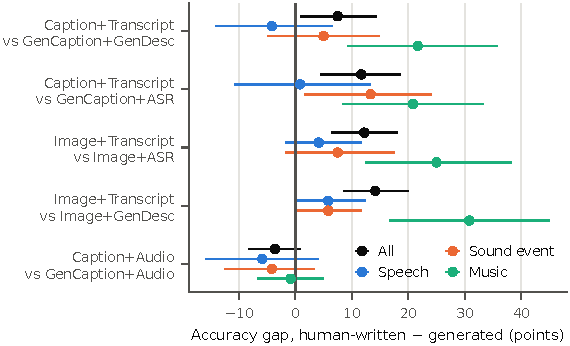
\includegraphics[width=\columnwidth]{figures/idea4_paired_gaps.pdf}
\caption{Idea~4: paired accuracy gap between the reference and generated surrogates
(positive = generated is worse), overall and per audio type, with bootstrap 95\%
CIs.}
\label{fig:idea4-gaps}
\end{figure}

\paragraph{Generated audio text breaks the text route.} Replacing the reference
surrogates with generated ones costs 7.5 points for caption+transcript
($[0.8,14.4]$, $p{=}0.04$), 11.7 points with ASR as the transcript ($p{=}0.002$),
and 12.2 points for image+ASR versus image+transcript ($p{=}0.0002$;
\cref{tab:idea4,fig:idea4-gaps}). Almost all of the loss is on music ($-21.7$ points,
$p{=}0.006$); on speech, generated text is actually 4.2 points better (not
significant). The caption is not the problem: our generated caption with audio
matches the reference caption with audio (43.3\% vs.\ 39.7\%), even though the
reference captions come from a model about 25$\times$ larger. The failure is on the
audio side.

\begin{table}[t]
\caption{Idea~4 examples: human-written vs.\ generated audio surrogates (abridged).
The human descriptions name the exact entity the question asks about.}
\label{tab:idea4-examples}
\centering\scriptsize
\setlength{\tabcolsep}{2.5pt}
\begin{tabular}{p{0.15\columnwidth}p{0.38\columnwidth}p{0.40\columnwidth}}
\toprule
Item & Human-written & Generated (Qwen / Whisper) \\
\midrule
1047 music: which instrument? (ruan) & ``A \textbf{Ruan} (a Chinese lute) concerto performance with double bass and Chinese woodwinds'' & ``a \textbf{guitar} playing a fast-paced, upbeat melody'' / ASR: ``Thank you so much for joining us.'' \\
\addlinespace
1052 music: what do the instruments share? (both lutes) & ``A solo live recording of arabic \textbf{oud}, a traditional Middle Eastern lute'' & ``a solo \textbf{guitar} performance \ldots\ key of A minor'' / ASR: ``Thank you.'' \\
\addlinespace
895 sound: what is the man holding? (flare stick) & ``Sound of \textbf{fuse burning} + reaching the sky'' & ``an \textbf{explosion} followed by a whooshing sound'' / ASR: ``Oh, my God.'' \\
\bottomrule
\end{tabular}
\end{table}

\paragraph{Human descriptions leak the answer.} The reference text does so well on
music partly because the human audio descriptions often name the exact thing the
question asks about (``Ruan'', ``oud'', ``fuse burning''), while the generated
descriptions use generic words (``guitar'', ``explosion''; \cref{tab:idea4-examples}).
These descriptions act partly as labels rather than as summaries a perception model
could produce. Our Assignment~2 result that caption+transcript matches the raw input
is therefore an upper bound that assumes an expert describer.

\paragraph{Generated text is expensive.} A caption takes 5.3\,s and an audio
description 3.6\,s on average, so the generated text route costs 8.9\,s per item,
about 25$\times$ the 0.36\,s needed to answer from the raw image and audio
(\cref{fig:idea4-cost}). It also processes more tokens (1,752 vs.\ 1,140), because
generating the text requires encoding the raw inputs anyway. Only Whisper is cheap
(0.46\,s). Text surrogates save computation only if they already exist or are reused
across many questions about the same input.

\begin{figure}[t]
\centering
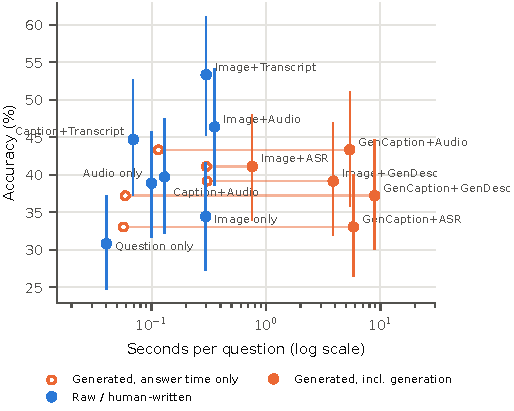
\includegraphics[width=\columnwidth]{figures/idea4_acc_vs_total_cost.pdf}
\caption{Idea~4: test accuracy vs.\ total cost per item, including surrogate
generation. Every generated configuration is both less accurate and more expensive
than answering from the raw image and audio.}
\label{fig:idea4-cost}
\end{figure}

\begin{figure}[t]
\centering
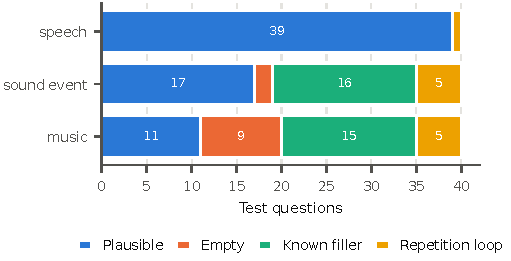
\includegraphics[width=\columnwidth]{figures/idea4_asr_status.pdf}
\caption{Whisper output category on the test audio. Outside speech, most clips
yield empty output, a known filler phrase, or a repetition loop.}
\label{fig:idea4-asr}
\end{figure}

\paragraph{Failure analysis.} (i) \emph{Whisper invents text for non-speech audio.}
It is reliable on speech (39 of 40 clips), but on 52 of the 80 sound and music clips
it returns nothing (11), a stock phrase such as ``Thank you so much for joining us''
(31), or a repeating loop (10)~\citep{koenecke2024careless}; see \cref{fig:idea4-asr}.
On music clips where it loops, image+ASR is right 6.7\% of the time, versus 86.7\%
with the human description. (ii) \emph{Perception is wrong or too generic.} In item
1047, a ruan (a Chinese lute) appears in both the image and the audio. The generated
caption says ``a traditional Chinese musical instrument'' and the audio description
says ``a guitar playing a fast-paced, upbeat melody''; the model picks the wrong
instrument in all three orders, while the reference surrogates get it right. For
speech, descriptions sometimes leave out the key words (item 988: ``a male voice
speaking \ldots\ neutral mood''). (iii) \emph{Generation is hard to control.} In our
first run, without an explicit stop at the end of the turn, Qwen kept going, invented
``Human:'' turns, and ended in repeated text in another language, so every surrogate
hit the token limit. Even after the fix, outputs end with chat phrases such as
``What do you think about this audio clip?'', which shows that the model treats
describing as chatting. A separate run of the same pipeline on the M2 Max agrees
with the L4 run on 81\% of predictions, with accuracies within 4 points, so these
results are not hardware artifacts.

\subsection{Updated Research Idea}

Text surrogates help when they contain the deciding information, as the human music
and sound descriptions do, not because text is inherently cheaper. For the final
report we will (a) \emph{match the surrogate to the audio type}: send speech to ASR
and other audio to an audio-captioning or tagging model, and fall back to raw audio
when the ASR output looks broken (empty, filler, looping, or low log-probability);
(b) \emph{condition the surrogate on the question}, so it describes only what the
question asks about, and compare this with the question-agnostic baseline; and (c)
\emph{share the generation cost} across the $k$ questions asked about the same input,
$C=C_{\text{ans}}+C_{\text{gen}}/k$, and find the break-even $k$ at which generated
text becomes cheaper than the raw inputs. The ASR-failure detector also becomes a
feature for the Idea~1 router.

In course terms, Idea~4 studies \emph{modality translation}: translating audio or
images into text loses information in ways that depend on the source, working for
speech but staying generic for music and sounds. We will measure translation quality
directly, as overlap with the human text and whether the answer entity is mentioned,
and relate it to accuracy. We will also test the human descriptions with the answer
entity masked, to see whether text helps because it is easier to reason over or only
because it contains the answer.

% ===========================================================================
\section{Discussion and Next Steps}
\label{sec:discussion}

Cheap substitutes work only in specific cases: reference text but not text
generated at test time (Idea~4), small images and cut audio but not sped-up audio
(Idea~3), and per-item choices that a simple router cannot yet make (Idea~1). In
each case the deciding evidence sits in one modality, the cheaper input silently
drops it, and the model stays confident. Our final-report methods will therefore
share two parts: a cheap first pass that detects cross-modal disagreement and broken
surrogates, and a per-item policy trained on order-robust, relative targets. We will
keep averaging over option orders, since single-order accuracy on OmniBench
misranks configurations.

\paragraph{Limitations.} Our test sets are small (120 and 90 items, 30--40 per audio
type), so per-type differences under about 8 points are not reliable, and Idea~3
uses a different test set from Ideas~1 and~4. All results come from one 3B model;
larger models may use raw audio better. Three option orders remove most but not all
of the position bias: question-only accuracy on music stays at 41--52\%. Cost is
measured mainly in tokens and wall time on different hardware, and peak memory on
the M2 Max is approximate, so we do not compare memory across devices.

\bibliography{references,references_midterm}
\bibliographystyle{icml2026}

% ===========================================================================
\clearpage
\appendix

\section{AI/LLM Usage Disclosure}

\textbf{[Team: review and complete; this must describe all AI use accurately.]}

\begin{itemize}
  \item \textbf{Arjun Shah and Lindy Zhang} used Claude Code (Anthropic, Claude Opus
    5.5) throughout their midterm work: planning the experiments and splits; writing
    and debugging most of the code for the shared pipeline, the Idea~1 router, the
    Idea~3 time-stretching ablation, and the local Idea~4 replication; running the
    analyses; diagnosing failures (a decoding error on one audio file, and the
    generation not stopping at the end of a turn); and drafting this report from the
    computed results. Arjun and Lindy chose the ideas and experimental design,
    launched and monitored all runs, checked the outputs, and revised the text.
  \item \textbf{Alvin Wang} (Idea~3) and \textbf{Nikkita Batra} (Idea~4):
    \textbf{[describe any AI use in your code, analysis, and writing]}.
  \item No AI model produced or altered any experimental results.
\end{itemize}

\section{Teammate Contributions}

\begin{itemize}
  \item \textbf{Arjun Shah and Lindy Zhang} worked together on: the shared
    experimental pipeline (data split, option-order averaging, extended runner for
    budget and surrogate configurations, audio-decoding fix); all 6,300 Idea~1 model
    runs on the M2 Max; the Idea~1 router baseline, its evaluation, and its failure
    analysis; the Idea~3 time-stretching ablation (5,760 runs); and an independent
    Idea~4 replication on the M2 Max (generation and 1,800 scoring runs).
  \item \textbf{Alvin Wang} designed and implemented the Idea~3 budget-grid baseline
    (runner, PSC/V100 job scripts, 10,800 runs), the analysis (marginal utility,
    Shapley attribution, dev-selected policies, cross-hardware agreement check), and
    the Idea~3 failure analysis and section.
  \item \textbf{Nikkita Batra} designed and implemented the Idea~4 generated-surrogate
    pipeline and analysis (Whisper ASR and Qwen captions and descriptions,
    generation-cost accounting, ASR failure categories, paired comparisons), ran it
    on an L4 GPU, and produced the Idea~4 results and failure examples.
  \item \textbf{All four authors} wrote and revised the report.
\end{itemize}

\end{document}
